% questions.tex —— 2017 年·上海普通高考卷 · 题目内容片段（无答案）
% 由 tools/generate_projects.py 依来源总账自 2017/2017_数学真题_上海_试题.md 生成，勿手改（改源 MD 后重跑）


\begin{gktip}
\textbf{来源与核对边界}：题面依据来源清单固定文件的 PDF 第 1–2 页转录。该文件页眉自题“2017 普通高等学校招生考试（上海卷）”；发布者、出版物、版次及原始来源链未核实；固定输入已在本库内部绑定到 \texttt{gk-2017-regular-shanghai}，不构成来源认证。固定文件只有题面页，没有答案、解析或评分材料；本文件不含答案，也不据此声称官方身份。

\textbf{图形}：源 PDF 第 1 页的第 7、12、17 题含图；第 2 页 Q20 题干后没有图。以下 TikZ 图按固定来源结构和标注重绘，不从示意图比例添加题设条件。
\end{gktip}

\gkpart{一、填空题}

\begin{question}
\gkti{1}已知集合 $A=\{1,2,3,4\}$，集合 $B=\{3,4,5\}$，则 $A\cap B=\underline{\qquad}$。

\end{question}
\begin{question}
\gkti{2}若排列数 $P_6^m=6\times5\times4$，则 $m=\underline{\qquad}$。

\end{question}
\begin{question}
\gkti{3}不等式 $\dfrac{x-1}{x}>1$ 的解集为 $\underline{\qquad}$。

\end{question}
\begin{question}
\gkti{4}已知球的体积为 $36\pi$，则该球主视图的面积等于 $\underline{\qquad}$。

\end{question}
\begin{question}
\gkti{5}已知复数 $z$ 满足 $z+\dfrac{3}{z}=0$，则 $|z|=\underline{\qquad}$。

\end{question}
\begin{question}
\gkti{6}设双曲线 $\dfrac{x^2}{9}-\dfrac{y^2}{b^2}=1\ (b>0)$ 的焦点为 $F_1,F_2$，$P$ 为该双曲线上的一点，若 $|PF_1|=5$，则 $|PF_2|=\underline{\qquad}$。

\Needspace{0.4\textheight}
\end{question}
\begin{question}
\gkti{7}如图，以长方体 $ABCD-A_1B_1C_1D_1$ 的顶点 $D$ 为坐标原点，过 $D$ 的三条棱所在的直线为坐标轴，建立空间直角坐标系。若 $\overrightarrow{DB_1}$ 的坐标为 $(4,3,2)$，则 $\overrightarrow{AC_1}$ 的坐标是 $\underline{\qquad}$。
\nopagebreak[4]
\begin{center}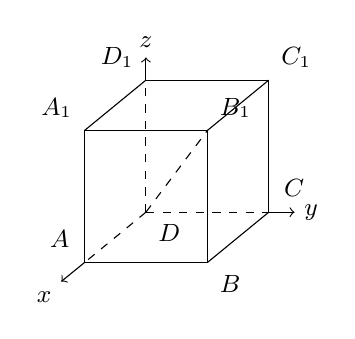
\begin{tikzpicture}[x=0.78cm,y=0.78cm,every node/.style={font=\small}]
  % Source-faithful cuboid topology; projection lengths are schematic.
  \coordinate (D)  at (0,0);
  \coordinate (A)  at (-1.0,-0.82);
  \coordinate (C)  at (2.0,0);
  \coordinate (B)  at (1.0,-0.82);
  \coordinate (D1) at (0,2.15);
  \coordinate (A1) at (-1.0,1.33);
  \coordinate (C1) at (2.0,2.15);
  \coordinate (B1) at (1.0,1.33);

  % Visible cuboid edges.
  \draw (A) -- (B);
  \draw (B) -- (C);
  \draw (A) -- (A1);
  \draw (B) -- (B1);
  \draw (C) -- (C1);
  \draw (A1) -- (B1);
  \draw (B1) -- (C1);
  \draw (C1) -- (D1);
  \draw (D1) -- (A1);

  % Hidden cuboid edges along the three coordinate axes.
  \draw[dashed] (D) -- (A);
  \draw[dashed] (D) -- (C);
  \draw[dashed] (D) -- (D1);

  % The source also shows the vector DB_1 as a dashed diagonal.
  \draw[dashed] (D) -- (B1);

  % Positive coordinate directions continue beyond the corresponding vertices.
  \draw[->] (A) -- (-1.38,-1.13) node[below left] {$x$};
  \draw[->] (C) -- (2.42,0) node[right] {$y$};
  \draw[->] (D1) -- (0,2.52) node[above] {$z$};

  \node[below right=1pt] at (D) {$D$};
  \node[above left=2pt] at (A) {$A$};
  \node[below right=1pt] at (B) {$B$};
  \node[above right=2pt] at (C) {$C$};
  \node[above left=1pt] at (D1) {$D_1$};
  \node[above left=1pt] at (A1) {$A_1$};
  \node[above right=1pt] at (B1) {$B_1$};
  \node[above right=1pt] at (C1) {$C_1$};
\end{tikzpicture}
\end{center}
\nopagebreak[4]
\end{question}
\begin{question}
\gkti{8}定义在 $(0,+\infty)$ 上的函数 $y=f(x)$ 的反函数为 $y=f^{-1}(x)$。若
\nopagebreak[4]
\[
g(x)=
\begin{cases}
3^x-1,&x\leqslant0,\\
f(x),&x>0,
\end{cases}
\]
为奇函数，则 $f^{-1}(x)=2$ 的解为 $\underline{\qquad}$。

\end{question}
\begin{question}
\gkti{9}已知四个函数：① $y=-x$，② $y=-\dfrac1x$，③ $y=x^3$，④ $y=x^{\frac12}$。从中任选 2 个，则事件“所选 2 个函数的图象有且仅有一个公共点”的概率为 $\underline{\qquad}$。

\end{question}
\begin{question}
\gkti{10}已知数列 $\{a_n\}$ 和 $\{b_n\}$，其中 $a_n=n^2$，$n\in\mathbb N^*$；$\{b_n\}$ 的项是互不相等的正整数。若对于任意 $n\in\mathbb N^*$，$\{b_n\}$ 的第 $a_n$ 项都等于 $\{a_n\}$ 的第 $b_n$ 项，则
\nopagebreak[4]
\[
\dfrac{\lg(b_1b_4b_9b_{16})}{\lg(b_1b_2b_3b_4)}=\underline{\qquad}\text{。}
\]

\end{question}
\begin{question}
\gkti{11}设 $\alpha_1,\alpha_2\in\mathbb R$，且
\nopagebreak[4]
\[
\dfrac{1}{2+\sin\alpha_1}+\dfrac{1}{2+\sin(2\alpha_2)}=2\text{，}
\]
则 $|10\pi-\alpha_1-\alpha_2|$ 的最小值等于 $\underline{\qquad}$。

\Needspace{0.4\textheight}
\end{question}
\begin{question}
\gkti{12}如图，用 35 个单位正方形拼成一个矩形，点 $P_1,P_2,P_3,P_4$ 以及四个标记为“$\blacktriangle$”的点在正方形的顶点处。设集合 $\Omega=\{P_1,P_2,P_3,P_4\}$，点 $P\in\Omega$，过 $P$ 作直线 $l_P$，使得不在 $l_P$ 上的“$\blacktriangle$”的点分布在 $l_P$ 的两侧。用 $D_1(l_P)$ 和 $D_2(l_P)$ 分别表示 $l_P$ 一侧和另一侧的“$\blacktriangle$”的点到 $l_P$ 的距离之和。若过 $P$ 的直线 $l_P$ 中有且只有一条满足 $D_1(l_P)=D_2(l_P)$，则 $\Omega$ 中所有这样的 $P$ 为 $\underline{\qquad}$。
\nopagebreak[4]
\begin{center}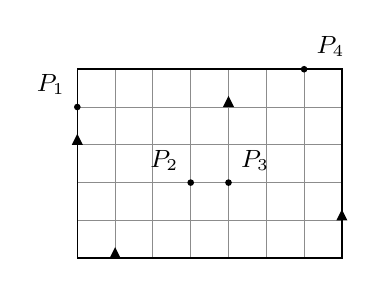
\begin{tikzpicture}[x=0.48cm,y=0.48cm,every node/.style={font=\small}]
  % Seven columns by five rows of unit squares; coordinates are only for redraw.
  \draw[step=1,black!45,line width=0.35pt] (0,0) grid (7,5);
  \draw[line width=0.55pt] (0,0) rectangle (7,5);

  % Marked P-points from the source.
  \fill (0,4) circle (1.2pt);
  \node[above left=1pt] at (0,4) {$P_1$};
  \fill (3,2) circle (1.2pt);
  \node[above left=1pt] at (3,2) {$P_2$};
  \fill (4,2) circle (1.2pt);
  \node[above right=1pt] at (4,2) {$P_3$};
  \fill (6,5) circle (1.2pt);
  \node[above right=1pt] at (6,5) {$P_4$};

  % The four solid triangles occupy the source lattice vertices.
  \fill (1,0) ++(-2pt,0) -- ++(2pt,4pt) -- ++(2pt,-4pt) -- cycle;
  \fill (0,3) ++(-2pt,0) -- ++(2pt,4pt) -- ++(2pt,-4pt) -- cycle;
  \fill (4,4) ++(-2pt,0) -- ++(2pt,4pt) -- ++(2pt,-4pt) -- cycle;
  \fill (7,1) ++(-2pt,0) -- ++(2pt,4pt) -- ++(2pt,-4pt) -- cycle;
\end{tikzpicture}
\end{center}
\nopagebreak[4]
\end{question}
\gkpart{二、选择题}

\begin{question}
\gkti{13}关于 $x,y$ 的二元一次方程组
\nopagebreak[4]
\[
\begin{cases}
x+5y=0,\\
2x+3y=4,
\end{cases}
\]
的系数行列式 $D$ 为（　）。

（A）$\begin{vmatrix}0&5\\4&3\end{vmatrix}$　（B）$\begin{vmatrix}1&0\\2&4\end{vmatrix}$　（C）$\begin{vmatrix}1&5\\2&3\end{vmatrix}$　（D）$\begin{vmatrix}6&0\\5&4\end{vmatrix}$

\end{question}
\begin{question}
\gkti{14}在数列 $\{a_n\}$ 中，$a_n=\left(-\dfrac12\right)^n$，$n\in\mathbb N^*$，则 $\displaystyle\lim_{n\to\infty}a_n$（　）。

（A）等于 $-\dfrac12$　（B）等于 $0$　（C）等于 $\dfrac12$　（D）不存在

\end{question}
\begin{question}
\gkti{15}已知 $a\text{、}b\text{、}c$ 为实常数，数列 $\{x_n\}$ 的通项 $x_n=an^2+bn+c$，$n\in\mathbb N^*$，则“存在 $k\in\mathbb N^*$，使得 $x_{100+k},x_{200+k},x_{300+k}$ 成等差数列”的一个必要条件是（　）。

（A）$a\geqslant0$　（B）$b\leqslant0$　（C）$c=0$　（D）$a-2b+c=0$

\end{question}
\begin{question}
\gkti{16}在平面直角坐标系 $xOy$ 中，已知椭圆 $C_1:\dfrac{x^2}{36}+\dfrac{y^2}{4}=1$ 和 $C_2:x^2+\dfrac{y^2}{9}=1$。$P$ 为 $C_1$ 上的动点，$Q$ 为 $C_2$ 上的动点，$w$ 是 $\overrightarrow{OP}\cdot\overrightarrow{OQ}$ 的最大值。记
\nopagebreak[4]
\[
\Omega=\{(P,Q)\mid P\text{ 在 }C_1\text{ 上，}Q\text{ 在 }C_2\text{ 上，且 }\overrightarrow{OP}\cdot\overrightarrow{OQ}=w\},
\]
则 $\Omega$ 中（　）。

（A）元素个数为 2　（B）元素个数为 4　（C）元素个数为 8　（D）含有无穷个元素

\end{question}
\gkpart{三、解答题}

\Needspace{0.4\textheight}
\begin{question}
\gkti{17}如图，直三棱柱 $ABC-A_1B_1C_1$ 的底面为直角三角形，两直角边 $AB$ 和 $AC$ 的长分别为 4 和 2，侧棱 $AA_1$ 的长为 5。

（1） 求三棱柱 $ABC-A_1B_1C_1$ 的体积；

（2） 设 $M$ 是 $BC$ 中点，求直线 $A_1M$ 与平面 $ABC$ 所成角的大小。
\nopagebreak[4]
\begin{center}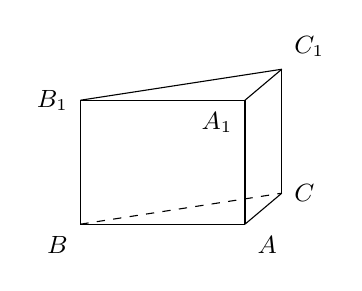
\begin{tikzpicture}[x=0.82cm,y=0.82cm,every node/.style={font=\small}]
  % Source-faithful triangular-prism topology; projection lengths are schematic.
  \coordinate (B)  at (0,0);
  \coordinate (A)  at (2.55,0);
  \coordinate (C)  at (3.12,0.48);
  \coordinate (B1) at (0,1.92);
  \coordinate (A1) at (2.55,1.92);
  \coordinate (C1) at (3.12,2.40);

  % Solid edges shown in the source diagram.
  \draw (B) -- (A);
  \draw (A) -- (C);
  \draw (A) -- (A1);
  \draw (B) -- (B1);
  \draw (C) -- (C1);
  \draw (B1) -- (A1);
  \draw (A1) -- (C1);
  \draw (B1) -- (C1);

  % The hidden base edge BC is dashed in the source.
  \draw[dashed] (B) -- (C);

  \node[below left=1pt] at (B) {$B$};
  \node[below right=1pt] at (A) {$A$};
  \node[right=1pt] at (C) {$C$};
  \node[left=1pt] at (B1) {$B_1$};
  \node[below left=1pt] at (A1) {$A_1$};
  \node[above right=1pt] at (C1) {$C_1$};
\end{tikzpicture}
\end{center}
\nopagebreak[4]
\end{question}
\begin{question}
\gkti{18}已知函数 $f(x)=\cos^2x-\sin^2x+\dfrac12$，$x\in(0,\pi)$。

（1） 求 $f(x)$ 的单调递增区间；

（2） 设 $\triangle ABC$ 为锐角三角形，角 $A$ 所对边 $a=\sqrt{19}$，角 $B$ 所对边 $b=5$。若 $f(A)=0$，求 $\triangle ABC$ 的面积。

\end{question}
\begin{question}
\gkti{19}根据预测，某地第 $n$（$n\in\mathbb N^*$）个月共享单车的投放量和损失量分别为 $a_n$ 和 $b_n$（单位：辆），其中
\nopagebreak[4]
\[
a_n=
\begin{cases}
5n^4+15,&1\leqslant n\leqslant3,\\
-10n+470,&n\geqslant4,
\end{cases}
\qquad b_n=n+5\text{，}
\]
第 $n$ 个月底的共享单车的保有量是前 $n$ 个月的累计投放量与累计损失量的差。

（1） 求该地区第 4 个月底的共享单车的保有量；

（2） 已知该地共享单车停放点第 $n$ 个月底的单车容纳量 $S_n=-4(n-46)^2+8800$（单位：辆）。设在某月底，共享单车保有量达到最大，问该保有量是否超出了此时停放点的单车容纳量？

\end{question}
\begin{question}
\gkti{20}在平面直角坐标系 $xOy$ 中，已知椭圆 $\Gamma:\dfrac{x^2}{4}+y^2=1$，$A$ 为 $\Gamma$ 的上顶点，$P$ 为 $\Gamma$ 上异于上、下顶点的动点，$M$ 为 $x$ 轴正半轴上的动点。

（1） 若 $P$ 在第一象限，且 $|OP|=\sqrt2$，求 $P$ 的坐标；

（2） 设 $P\left(\dfrac85,\dfrac35\right)$，若以 $A\text{、}P\text{、}M$ 为顶点的三角形是直角三角形，求 $M$ 的横坐标；

（3） 若 $|MA|=|MP|$，直线 $AQ$ 与 $\Gamma$ 交于另一点 $C$，且 $\overrightarrow{AQ}=2\overrightarrow{AC}$，$\overrightarrow{PQ}=4\overrightarrow{PM}$，求直线 $AQ$ 的方程。

\begin{gktip}
\textbf{转录边界}：Q20（3）按源文保留关于点 $Q$ 的两组向量关系。独立解析由这些关系与其余条件确定 $Q$，未增补题设条件。
\end{gktip}

\end{question}
\begin{question}
\gkti{21}设定义在 $\mathbb R$ 上的函数 $f(x)$ 满足：对于任意的 $x_1,x_2\in\mathbb R$，当 $x_1<x_2$ 时，都有 $f(x_1)\leqslant f(x_2)$。

（1） 若 $f(x)=ax^3+1$，求 $a$ 的取值范围；

（2） 若 $f(x)$ 是周期函数，证明：$f(x)$ 是常值函数；

（3） 设 $f(x)$ 恒大于零。$g(x)$ 是定义在 $\mathbb R$ 上的、恒大于零的周期函数，$M$ 是 $g(x)$ 的最大值。函数 $h(x)=f(x)g(x)$。证明：“$h(x)$ 是周期函数”的充要条件是“$f(x)$ 是常值函数”。

\end{question}